%%%%%%%%%%%%%%%%%%%%%%%%%%%%%%%%%%%%%%%%%%%%%%%%%%%%%%%%%%%%%%%%%%% 
%                                                                 %
%                            CHAPTER                              %
%                                                                 %
%%%%%%%%%%%%%%%%%%%%%%%%%%%%%%%%%%%%%%%%%%%%%%%%%%%%%%%%%%%%%%%%%%% 
\chapter{Implementation}
\label{chapter:implementation}
This chapter is split into three sections. In the first section, we go over the structure of the algorithm. In the second and third sections, we go into detail about the two sub-research questions: how to construct the schema and how to populate the schema. 


% At this time we only have a PoC implementation, as such many details haven't been worked out yet. For example, the section on creating the schema is limited, as we only handle CSV files which require little to no schema. 

For the implementation, we assume that the mapping rules never map to a superset of the knowledge graph. 

The implementation is written in Python. As we seek to extend Morph-KGC we make use of its internal functions and the libraries to work with those, like pandas. Querying the knowledge graph is done with the SPARQLWrapper library.

\section{General structure}
The algorithm consists of 4 main parts: setting up, creating the schema, retrieving the data, and applying the data to the schema. Creating the schema and retrieving the data are the two main parts of the implementation, and are covered in their sections. Setting up consists of setting up the \acrshort{sparql} endpoint if necessary and processing the mapping files. Applying the data to the schema consists of applying the data of each iteration to the schema, and creating the output file. A graphical representation of the algorithm can be found in figure \ref{fig:algorithm}. A more formal representation can be found in algorithm \ref{alg:inversion}.

\begin{figure}[h]
    \centering
    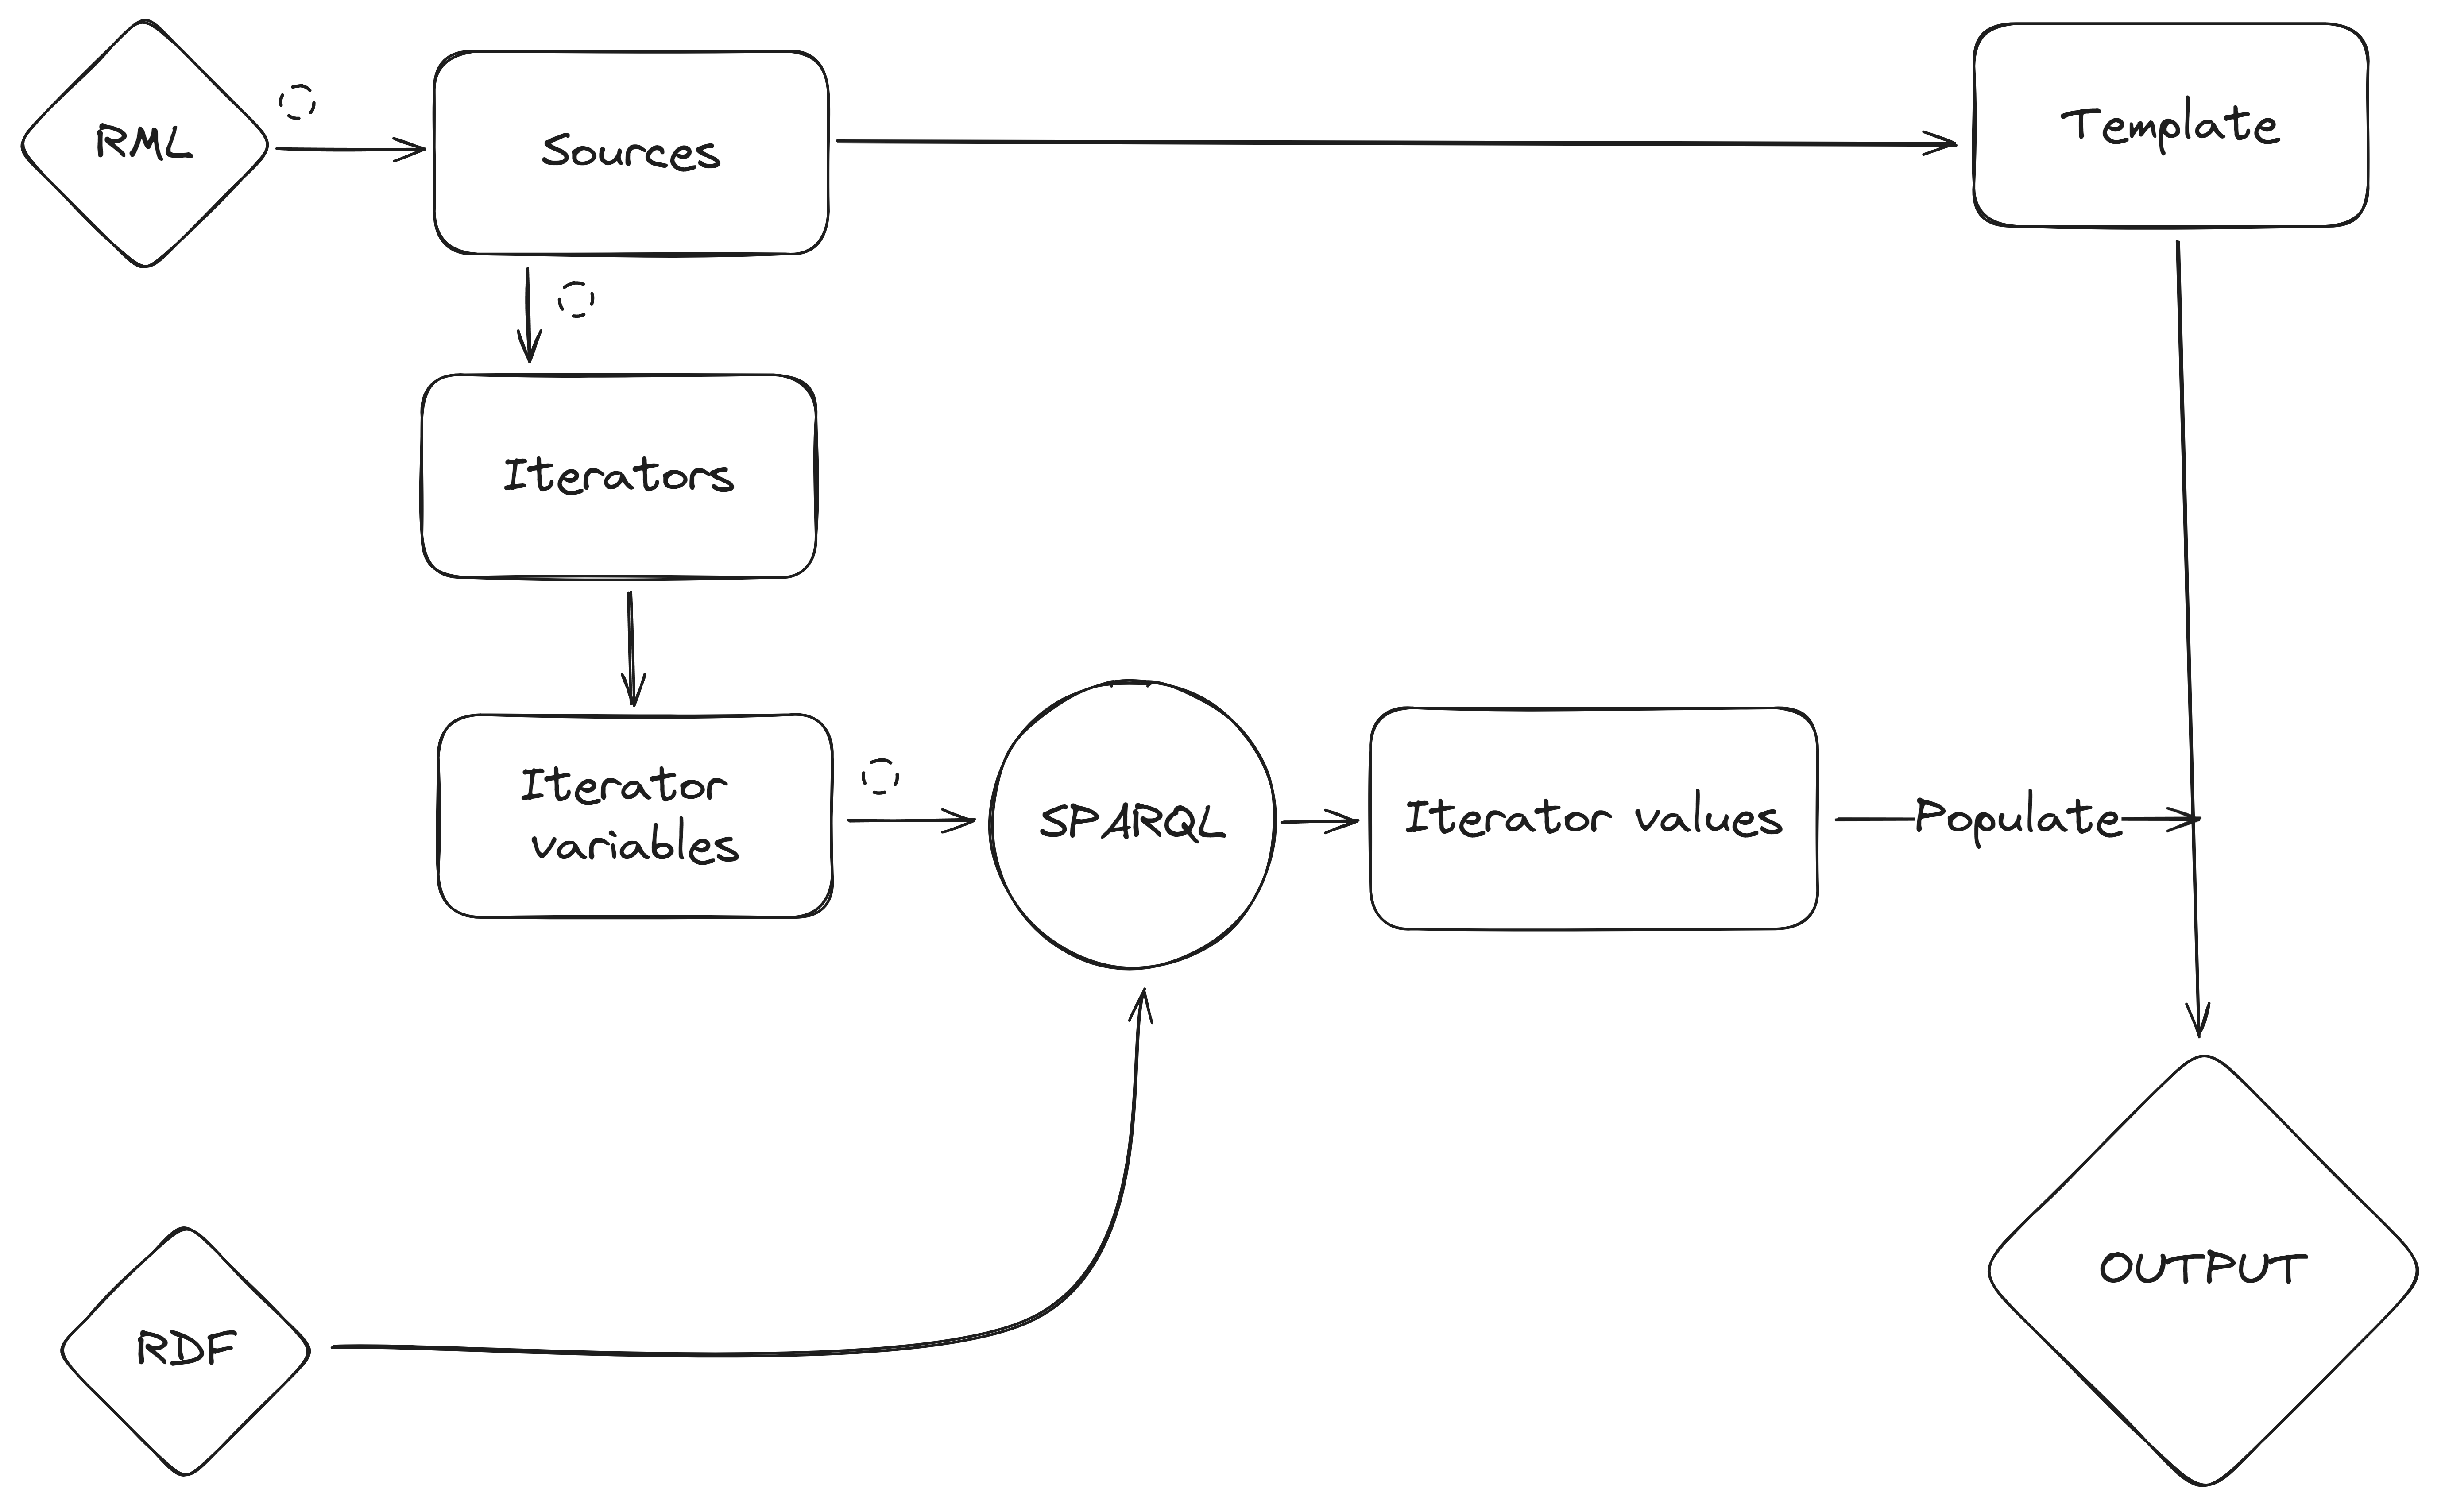
\includegraphics[width=\textwidth]{Chapter3/algorithm_flat.png}
    \caption{Overview of the algorithm}
    \label{fig:algorithm}
\end{figure}

\begin{algorithm}
    \caption{Inversion}
    \label{alg:inversion}
    \begin{algorithmic}[1]
        \State $optional(graph \gets load\_graph(rdf))$
        \Require{$mapping\_files$ is a set of mapping files}
        \Require{$graph$ is a sparql endpoint}
        \ForAll{$mapping\_file \in mapping\_files$}
            \State $mapping\_rules \gets parse\_mapping\_file(mapping\_file)$
        \EndFor
        \ForAll{$source, source\_rules \in mapping\_rules.groupby('source')$}
            \ForAll{$iterator, iterator\_rules \in source\_rules.groupby('iterator')$}
                \State $selected\_rules \gets get\_optimal\_rules(iterator\_rules)$
                \ForAll{$subject, subject\_rules \in selected\_rules.groupby('subject')$}
                    \State $query \gets generate\_query(subject\_rules)$
                    \State $values[iterator] \gets graph.query(query)$
                \EndFor
            \EndFor
            \State $templates \gets generate\_templates(source\_rules)$
            \State $source\_output \gets apply\_templates(templates, values)$
        \EndFor
    \end{algorithmic}
\end{algorithm}

\subsection{Loading the mapping rules}
We start by loading the mapping rules from the mapping files. We use Morph-KGC's internal \texttt{retrieve\_mappings} function for this. This function takes a config file (.ini format) as input, which specifies the location of the mapping files and various other settings for which we have little use as they are only used for the materialization process. When relevant later on we could add our settings to this config file.
The mappings are returned as a pandas DataFrame. As the pandas library has the functionality to group by columns, we can easily group the mapping rules by source and iterator later. An example of a single mapping rule (row in the DataFrame) can be found in listing \ref{lst:mapping_rule}.

\begin{lstlisting}[caption={Example of a mapping rule in Morph-KGC}, label={lst:mapping_rule}, captionpos=b, basicstyle=\small]
    source_name: DataSource1 
    triples_map_id: #TM0
    triples_map_type: http://w3id.org/rml/TriplesMap
    logical_source_type: http://w3id.org/rml/source
    logical_source_value: student.csv
    iterator: nan
    subject_map_type: http://w3id.org/rml/template
    subject_map_value: http://example.com/{Name}
    subject_termtype: http://w3id.org/rml/IRI
    predicate_map_type: http://w3id.org/rml/constant
    predicate_map_value: http://xmlns.com/foaf/0.1/name
    object_map_type: http://w3id.org/rml/reference
    object_map_value: Name
    object_termtype: http://w3id.org/rml/Literal
    object_datatype: nan
    object_language: nan
    graph_map_type: http://w3id.org/rml/constant
    graph_map_value: http://w3id.org/rml/defaultGraph
    subject_join_conditions: nan
    object_join_conditions: nan
    source_type: CSV
    mapping_partition: 1-1-1-1
\end{lstlisting}

\section{Contructing the schema}
\label{section:constructing_schema}
Constructing the schema is done by reversing the mapping rules' source. We do this using the iterator and the mapping rule's references. \acrshort{rml} supports many different types of sources and referenceFormulations. We will implement the CSV, xPath, and JSONPath referenceFormulations. Not every source is a file, so for query-based sources, we will generate the query output. In a later stage, we could look into taking it a step further, generating the actual source behind those intermediate results.

As each referenceFormulation has its reference syntax, we will have to tailor the implementation to each referenceFormulation. For the PoC, we only implement the CSV referenceFormulation. 

\subsection{CSV}
\label{subsection:csv}
The CSV referenceFormulation is the simplest of the three as it describes a simple two-dimensional table, with columns having the names of the references and rows being the iterated values. The example TriplesMap in listing \ref{lst:csv_file_mapping} results in the CSV template in listing \ref{lst:csv_file}. Unlike the other referenceFormulations, CSV has no uncertainty in terms of structure.

\begin{lstlisting}[caption={Example mapping for a CSV file}, label={lst:csv_file_mapping}, captionpos=b, basicstyle=\small]
<TriplesMap1> a rr:TriplesMap;

rml:logicalSource [ 
    rml:source "student.csv";
    rml:referenceFormulation ql:CSV
];

rr:subjectMap [ 
    rr:template "http://example.com/Student/{ID}/{Name}";
    rr:graph ex:PersonGraph ;
    rr:class foaf:Person
];
\end{lstlisting}

\begin{lstlisting}[caption={Example CSV template}, label={lst:csv_file}, captionpos=b, basicstyle=\small]
ID,Name
<id>,<name>
\end{lstlisting}

\section{Retrieving the data}
TODO: add this section